\chapter{Methodology}
In this chapter, the cost function would be defined at first. Then, owing to its importance,  different methods of calculating resistance would be introduced. In final, the theory about path planning would be announced. However, in this chapter, only theories would be shown. In programming process, these methods or equations would be modified based on some assumptions, which would be elaborated in \autoref{progprocess}.
\section{Cost calculating}
In this project, we could estimate the cost function as the energy needed for a path. So, the cost function could be stated as:
\begin{equation}
    C=\int_{0}^{t} P(t) dt
    \label{cost fun}
\end{equation}
\begin{itemize}
    \item $C$: Cost of voyage
    \item $P$: Power of ship engine
    \item $t$: Time needed in this task
\end{itemize}
As we known, there will be resistance when the ship moves forward. To keep the desired velocity, we need thrust to counteract this resistance and the effective power of ship engine could be given as:
\begin{equation}
    P_{E}=T_{e}*V_{G}=R*V_{G}
    \label{ship power}
\end{equation}
\begin{itemize}
    \item $P_{E}$: Effective power of ship engine
    \item $T_{e}$: Effective thrust
    \item $V_{G}$: Measured ship's speed over ground
    \item $R$: Resistance of shipping
\end{itemize}
Actually, this effective power $P_{E}$ is different from the power of engine $P$, whose relationship could be rewritten as:
\begin{equation}
    P_{E}=\eta P
\end{equation}
\begin{itemize}
    \item $\eta$: Conversion efficiency
\end{itemize}
This conversion efficiency would be affected by many factors like ship velocities, engine and shafting structure and work environment.
\\The resistance in Eq.(\ref{ship power}) is related to many parameters as well, like ship velocities, ship parameters and ocean conditions. It would be elaborated in \autoref{sec:resistance}.
\\On the other hand, the task time Eq.(\ref{cost fun}) is related with the path length and the ship velocity, so it could be written as:
\begin{equation}
    t=L_{path}/V_{G}
    \label{task time}
\end{equation}
\begin{itemize}
    \item $L_{path}$: Length of chosen path
\end{itemize}
In conclusion, the problem of this project could be modelled as that, an appropriate path whose length is $L_{i}$, and efficient ship velocities $V_{G,j}$ in each part of this path would be found to make the cost function of this voyage be minimum.
\begin{displaymath}
    \min_{i,j} C_{i,j}=f[P(R_{i,j},V_{G,j}),t(L_{path,i},V_{G,j})]
    \label{modelling}
\end{displaymath}

\section{Resistance}
\label{sec:resistance}
Ship is a kind of vehicle travelling between water and air, which means that the resistance of shipping could be classified as two parts based on different causes. The resistance $R_{wind}$ which caused by wind could be calculated by the ITTC recommended method. In some places, this resistance $R_{wind}$ could be considered as a part of added resistance, but in this project, it is split as an independent part because of its unique calculation method. The interaction between hull and calm water leads to bare-hull resistance $R_{hull}$, which consists many kinds of resistance, like viscous resistance, friction resistance and wave resistance. In this project, Hollenbach method was used to calculate $R_{hull}$. In addition, STAwave-1 was utilized to take added resistance caused by head waves $R_{wave}$ into this project.
\\So, in this project, the total resistance $R_{total}$ could be classified by these 3 independent parts:
\begin{equation}
    R_{total}=R_{wind}+R_{hull}+R_{wave}
    \label{R_total}
\end{equation}
\begin{itemize}
    \item $R_{total}$: Total resistance
    \item $R_{wind}$: Added resistance caused by wind
    \item $R_{hull}$: Bare-hull resistance in calm water, including viscous resistance, friction resistance and wave resistance
    \item $R_{wave}$: Added resistance caused by waves in advance
\end{itemize}
\subsection{Conventions}
It is important to define sign conventions, which could illustrate directions of ship, wave and wind. According to ITTC\cite{2017ITTC}, these conventions are shown as:
\begin{figure}[H]
    \centering
    \begin{subfigure}[c]{0.45\textwidth}
        \centering
        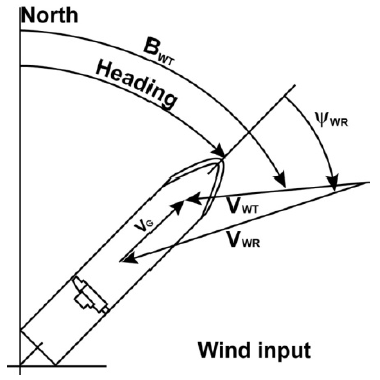
\includegraphics[width=\textwidth]{wind direction.png}
        \caption{Sign convention for wind directions}
        \label{wind directions}
    \end{subfigure}
    \begin{subfigure}[c]{0.45\textwidth}
        \centering
        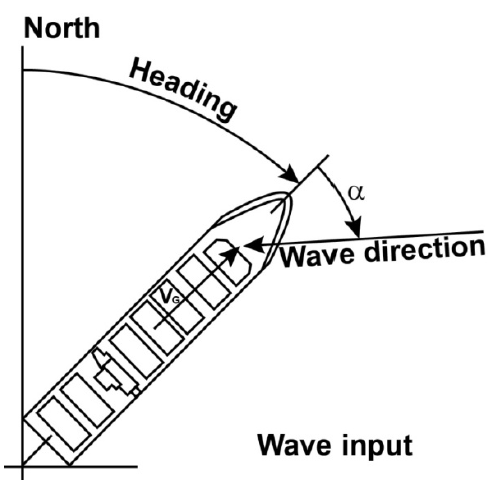
\includegraphics[width=\textwidth]{wave direction.png}
        \caption{Sign convention for wave directions}
        \label{wave directions}
    \end{subfigure}
    \caption{Sign conventions}
    \label{directions}
\end{figure}
\begin{itemize}
    \item $\psi$: Heading of the ship
    \item $V_{WR}$: Relative wind speed
    \item $\psi_{WR}$: Relative wind direction relative to the bow, ship fixed; 0 means head winds
    \item $V_{WT}$: True wind speed
    \item $B_{WT}$: True wind angle in earth system
    \item $\alpha$: Angle between ship heading and wave direction relative to the bow; 0 means head waves
\end{itemize}
The wind direction is defined as the direction from which the wind is coming and the wave direction is defined as the direction relative to the ship's heading from which the wave fronts are approaching.

\subsection{ITTC-Wind}
\label{sec:ITTC}
The air resistance will increase in line with how much of the hull is above waterline, and the relative velocity between the vessel and wind.
\\According to ITTC recommended guidelines\cite{2017ITTC}, the wind-induced resistance could be calculated by:
\begin{equation}
    R_{wind}=\frac{1}{2} \rho_{air} C_{D A}\left(\psi_{\text {WRref }}\right) A_{X V} V_{\text {WRref }}^{2}-\frac{1}{2} \rho_{A} C_{D A}(0) A_{X V} V_{G}^{2}
    \label{wind}
\end{equation}
\begin{itemize}
    \item $A_{XV}$: Ship's area of maximum transverse section exposed to the wind
    \item $C_{D A}$: Wind resistance coefficient
    \item $\rho_{air}$: Mass density of air
    \item $V_{\text {WRref }}$: Relative wind speed at reference height
    \item $\psi_{\text {WRref }}$: Relative wind direction at reference height; 0 means heading wind
\end{itemize}
Data sets of the wind resistance coefficient $C_{x}$ depends on ship types and the relationship between $C_{x}$ and $C_{D A}$ is:
\begin{equation*}
    C_{x}=-C_{D A}
\end{equation*}
\begin{itemize}
    \item $C_{x}$: Data sets of the wind resistance coefficient
\end{itemize}
So, Eq.(\ref{wind}) could be rewritten as:
\begin{equation}
    R_{wind}=-\frac{1}{2} \rho_{A} C_{x}\left(\psi_{\text {WRref }}\right) A_{X V} V_{\text {WRref }}^{2}+\frac{1}{2} \rho_{A} C_{x}(0) A_{X V} V_{G}^{2}
    \label{wind1}
\end{equation}
The relative wind velocity at the reference height $V_{\text {WRref }}$ in Eq.(\ref{wind1}) could be given by:
\begin{equation*}
    V_{\text {WRref }}=\sqrt{V_{\text {WTref }}^{2}+V_{\mathrm{G}}^{2}+2 V_{\text {WTref}} V_{\mathrm{G}} \cos \left(\psi_{\text {WT }}-\psi\right)}
\end{equation*}
The relative wind direction at the reference height $\psi_{\text {WRref }}$ in Eq.(\ref{wind1}) could be given by:
\begin{equation*}
    \begin{aligned}
        \text{If:} \quad &V_{\mathrm{G}}+V_{\mathrm{WTref}} \cos \left(\psi_{\mathrm{WT}}-\psi\right) \geq 0\\
        &\psi_{\mathrm{WRref}}=\tan ^{-1} \frac{V_{\mathrm{WTref}} \sin \left(\psi_{\mathrm{WT}}-\psi\right)}  {V_{\mathrm{G}}+V_{\mathrm{WTref}} \cos \left(\psi_{\mathrm{WT}}-\psi\right)} \\
        \text{If:} \quad &V_{\mathrm{G}}+V_{\mathrm{WTref}} \cos \left(\psi_{\mathrm{WT}}-\psi\right)<0\\
        &\psi_{\mathrm{WRref}}=\tan ^{-1} \frac{V_{\mathrm{WTref}} \sin \left(\psi_{\mathrm{WT}}-\psi\right)}{V_{\mathrm{G}}+V_{\mathrm{WTref}} \cos \left(\psi_{\mathrm{WT}}-\psi\right)}+180^{\circ}
    \end{aligned}
\end{equation*}

\subsection{Hollenbach}
\label{sec:Hollenbach}
To predict the resistance in the calm water, the velocity and main dimensions of vessel should be taken into account. There are many methods for calculation and Hollenbach is the most recent empirical method for commercial vessels, which could estimate viscous resistance, friction resistance and wave resistance. This method is based on regression analysis of 433 ship models, and its calculation deeply depends on the vessels main dimensions\cite{HollenbachK1998EstimatingRA}.
\\Hollenbach method should be start with introducing the total resistance $R_{Tmean}$ caused by the reaction between hull and calm water, including viscous resistance, friction resistance and wave resistance. The viscous resistance and wave resistance could be consider as the residual resistance. So, $R_{Tmean}$ could be expressed as:
\begin{equation}
    \begin{aligned}
        R_{Tmean}&=R_{Fm}+R_{R}
        &=\frac{\rho_{sea}}{2} V_{G}^{2} \cdot\left(C_{F m} \cdot S+C_{R} \cdot B \cdot T\right)
    \end{aligned}
    \label{total resistance}
\end{equation}
\begin{itemize}
    \item $R_{Tmean}$: Mean total resistance, which caused by the reaction between hull and calm water
    \item $R_{Fm}$: (mean) Friction resistance
    \item $R_{R}$: Residual resistance
    \item $\rho_{sea}$: Mass density of sea water
    \item $C_{Fm}$: (mean) Friction resistance coefficient
    \item $S$: Wetted surface of ship
    \item $C_{R}$: Residual resistance coefficient
    \item $B$: Beam of ship
    \item $T$: Draft of ship
\end{itemize}
The (mean) friction resistance coefficient in Eq.(\ref{total resistance}) can be expressed as::
\begin{equation}
    C_{F}=\frac{0.075}{\left[\log \left(R_{e}\right)-2\right]^{2}}
\end{equation}
\begin{itemize}
    \item $R_{e}$: Reynold's number
\end{itemize}
Where:
\begin{equation*}
    R_{e}=\frac{V_{G} \cdot L}{\nu}
\end{equation*}
\begin{itemize}
    \item $L$: Vessel's length between perpendiculars
    \item $\nu$: Viscosity of sea water
\end{itemize}
By Hollenbach method, the residual coefficient $C_{R}$ in Eq.(\ref{total resistance}) can be expressed as:
\begin{equation}
    \begin{aligned}
        C_{R \text { Hollenbach }}=&C_{R, \text { Standard }} \cdot C_{R, F n K r i t} \cdot k_{L}  \\
        &\cdot\left(\frac{T}{B}\right)^{a 1} \cdot\left(\frac{B}{L}\right)^{a 2} \cdot\left(\frac{L_{O S}}{L_{w l}}\right)^{a 3} \cdot\left(\frac{L_{w l}}{L}\right)^{a 4} \\
        &\cdot\left(\frac{D_{p}}{T_{A}}\right)^{a 6} \cdot\left[1-\frac{T_{A}-T_{F}}{L}\right]^{a 5} \cdot\left(1-N_{R u d}\right)^{a 7} \\
        &\cdot\left(1-N_{B r a c}\right)^{a 8} \cdot\left(1-N_{B o s s}\right)^{a 9} \cdot\left(1-N_{T h r}\right)^{a 10}
        \label{CRH}
    \end{aligned}
\end{equation}
\begin{itemize}
    \item $L_{wl}$: Length of water line
    \item $T_{A}$: Draft of aft propeller
    \item $T_{F}$: Draft of fore propeller
    \item $D_{P}$: Propeller diameter
    \item $N_{R u d}$: Number of rudders
    \item $N_{\text {Brac }}$: Number of brackets
    \item $N_{\text {Boss }}$: Number of bossings
    \item $N_{T h r}$: Number of side thrusters
\end{itemize}
$C_{R, \text { Standard }}$ in Eq.(\ref{CRH}) is defined as:
\begin{equation}
    \begin{aligned}
        C_{R, \text { Standard }}=&b_{11}+b_{13} \cdot F_{n}+b_{13} \cdot F_{n}^{2}+C_{B} \cdot\left(b_{21}+b_{22} \cdot F_{n}+b_{23} \cdot F_{n}^{2}\right)\\
        &+C_{B}^{2} \cdot\left(b_{31}+b_{32} \cdot F_{n}+b_{33} \cdot F_{n}^{2}\right)
    \end{aligned}
    \label{CRS}
\end{equation} 
\begin{itemize}
    \item $C_{B}$: Block coefficient
\end{itemize}
Where:
\begin{equation*}
    C_{B}=\frac{\Delta}{L \cdot B \cdot T}
\end{equation*}
\begin{itemize}
    \item $\Delta$: Displacement, and only in above equation $\Delta$ represents displacement
\end{itemize}
\begin{equation*}
    F_{n}=\frac{V_{G}}{\sqrt{g \cdot L_{f n}}}
    \label{froudesnumber}
\end{equation*}
\begin{itemize}
    \item $F_{n}$: Froudes number
    \item $L_{f n}$: Froudes length
    \item $g$: Gravitational acceleration
\end{itemize}
However, the Froudes length is based on the value of the relation $L_{O S} / L$, where vessel's length over surface $L_{OS}$. According to Oosterveld's work \cite{oosterveld1975further}, $L_{O S}$, which is dependent on the loading condition, is defined as:
\begin{itemize}
    \item for design draught, is it the length between aft end of design waterline and the most forward point at the vessel below the design waterline.
    \item for ballast draught is it the length between aft end of the design and the forward end of the hull at ballast waterline.
\end{itemize}
The relation between $L_{O S} / L$ and $L_{f n}$ could be shown in following \autoref{FroudesL}:
\begin{table}[H]
    \begin{center}
        \caption{Definition of Froudes length: $L_{f n}$}
        \label{FroudesL}
        \begin{tabular}{c|c}
            \hline
            Values of $L_{O S} / L$ & Values of $L_{f n}$  \\ 
            \cline{1-2}
            $L_{O S} / L<1.0$          & $L_{O S}$                 \\ 
            \cline{1-2}
            $1.0<L_{O S} / L<1.1$   & $L+2 / 3 \cdot \left(L_{O S}-L\right)$\\ 
            \cline{1-2}
            $L_{O S} / L>1.1$          & $1.0667 \cdot L$   \\
            \hline   
        \end{tabular}
    \end{center}
\end{table}
\noindent $C_{R, F n K r i t}$ in Eq.(\ref{CRH}) is defined as:
\begin{equation}
    C_{R, F n K r i t}=\max \left[1.0,\left(\frac{F_{n}}{F_{n, k r i t}}\right)^{c_{1}}\right]
    \label{CRF}
\end{equation} 
$F_{n, k r i t}$ in above equation is:
\begin{equation}
    F_{n, k r i t}=d_{1}+d_{2} \cdot C_{B}+d_{3} \cdot F_{n}^{2}
    \label{Fnk}
\end{equation} 
$k_{L}$ in  Eq.(\ref{CRH}) is defined as:
\begin{equation}
    k_{L}=e_{1} \cdot L^{e 2}
    \label{kL}
\end{equation} 
These formulas are valid when Froudes number in following intervals:
\begin{equation}
    \begin{aligned}
        F_{n,\min }&=\min \left(f_{1}, f_{1}+f_{2}\left(f_{3}-C_{B}\right)\right) \\
        F_{n,\max }&=g_{1}+g_{2} C_{B}+g_{3} C_{B}^{3}
    \end{aligned}
    \label{FnI}
\end{equation}
If $F_{n}>F_{n,\max }$, the maximum resistance would be:
\begin{equation}
    R_{Tmax}=h_{1} \cdot R_{\text {Tmean }}
    \label{Rmax}
\end{equation}
If $F_{n}<F_{n,\min }$, $C_{R, F n K r i t}$ and $k_{L}$ in Eq.(\ref{CRH}) should be set to 1.0 for calculating the minimum resistance $R_{Tmin}$.
\\Coefficients $a \sim h$ in equations above: Eq.(\ref{CRH}), Eq.(\ref{CRS}), Eq.(\ref{CRF}), Eq.(\ref{Fnk}), Eq.(\ref{kL}) and Eq.(\ref{FnI}), could be found in Molland's work\cite{molland2011ship}.
\\In this project, $R_{hull}$ could be expressed as:
\begin{equation}
    R_{hull}=\left\{
        \begin{array}{rcl}
            R_{Tmin}     &      & F_{n}<F_{n,\min }\\
            R_{Tmean}  &      & F_{n,\min } \leq F_{n} \leq F_{n,\max }\\
            R_{Tmin}     &      & F_{n}>F_{n,\max }\\
        \end{array} \right.
    \label{RHullEq}
\end{equation}

\subsection{STAwave-1}
\label{sec:STAwave-1}
Parameters of wave and main dimensions of vessel should be taken into account, when we calculate the resistance caused by head waves. STAwave-1 is a correction method to estimate the added resistance in waves with limited input data.
\\As we stated, this method can be applied when a ship has limited pitch and heave. According to Boom's work \cite{van2013new},  this method is valid when the incoming wave are in the bow sector, within +/-45 degrees off the bow. Its formula is:
\begin{equation}
    R_{wave}=\frac{1}{16} \rho_{sea} g H_{\mathrm{W} 1 / 3}^{2} B \sqrt{\frac{B}{L_{\mathrm{BWL}}}}
    \label{STAwave}
\end{equation}
\begin{itemize}
    \item $H_{\mathrm{W} 1 / 3}$: Significant height of waves
    \item $L_{\mathrm{BWL}}$: Length of the bow on the water line to 95\% of maximum beam as shown in \autoref{LBWL}
\end{itemize}
\begin{figure}[H]  
	\centering  
	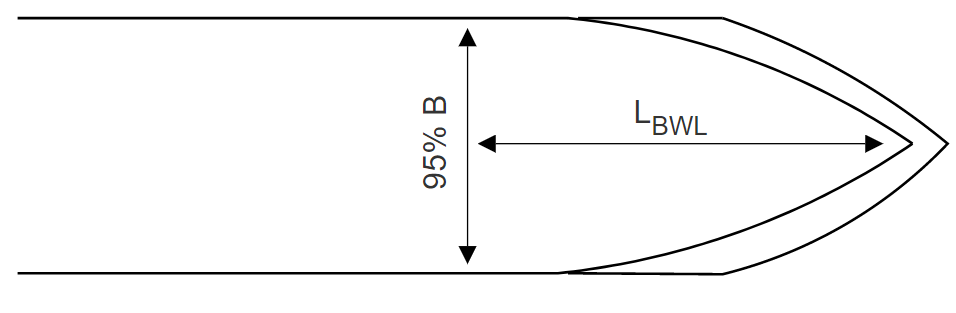
\includegraphics[width=0.9\linewidth]{definitionofLBWL.png}  
	\caption{Definition of $L_{\mathrm{BWL}}$}  
	\label{LBWL}  
\end{figure}
\section{Path planning}
Path planning, also named as motion planning, usually aims to find the shortest path, the path with lowest cost or the path who would take shortest time. One of the most popular methods to solve this shortest path problem is the Dijkstra algorithm, which is used in this project and the objective is to find the optimal route causing minimum fuel consumption.
\subsection{Dijkstra}
Dijkstra's algorithm, was conceived by the Dutch computer scientist Edsger Dijkstra\cite{dijkstra1959note}. Its basic thought is the process what from the start and gradually expand. In the process of exploring, record the path each to a point, and call the label. 
\\The origianl Dijkstra's algorithm will assign some initial distance values and will try to improve them step by step. However,in this project, the ship will move in the grids, and the distance between each coordinate point is equal (an assumption in Chapter 3) but the cost of going through are different. So, in this case, the node at the beginning of the path could be called as the origin node, and the toatl cost to go to the node Y could be defined as the cost from the origin node to Y. Then, the Dijkstra's algorithm would improve them step by step:
\begin{enumerate}[step 1]
    \item Mark all nodes unvisited. Create a set of all the unvisited nodes called the unvisited set.
    \item Assign to every node a cost value based on resistance. Set the initial node as current.
    \item For the current node, consider all of its unvisited neighbours and calculate their cost through the current node. Compare the newly calculated cost to the current assigned value and assign the lower one.
    \item When we are done considering all of the unvisited neighbours of the current node, mark the current node as visited and remove it from the unvisited set. A visited node will never be checked again.
    \item Stop if the destination node has been marked visited. The algorithm has finished.
    \item Otherwise, select the unvisited node that is marked with the lowest cost, set it as the new "current node", and go back to step 3.
\end{enumerate}
Based on these steps, a pseudocode algorithm could be shown as:
\begin{lstlisting}[caption= Pseudocode Dijkstra algorithm,label=Dijkstra]
    create US,VS
    while US is not empty:
        pick u_min in VS as u
        for each unvisited neighbour v of u:
            CC(v) = cost(u, v)
            if CC(v) < min cost(u, v):
                min cost(0,v) = CC(v)
        Ncost(v_min)=Ncost(u)+cost(u, v_min)
        if v_min == destination node:
            find EP
        else:
            removed v_min from US
            add v_min into VS
\end{lstlisting}
\begin{itemize}
    \item $US$: Unvisited set
    \item $VS$: Visited set
    \item $Ncost(u)$: Cost of the efficent path to node $u$
    \item $u_{min}$ Node who has min $Ncost(u)$
    \item $u$: Current node
    \item $cost(a,b)$: Cost of the path from node $a$ to node $b$
    \item $v$: Neighbour-nodes of $u$
    \item $CC(v)$: Current cost of the path from the original node to $v$ if it were to go through $u$
    \item $path(a,b)$: Current path from node $a$ to node $b$
    \item $v_{min}$: Neighbour-nodes of $u$, who has min $cost(u,v)$
    \item $EP$: Path to node destination node, whose cost equals to $Ncost(v_{min})$
\end{itemize}